\chapter{Umsetzung der interaktiven Benutzeroberfläche}
\label{chapter:umsetzung-der-interaktiven-benutzeroberfläche}

{\color{white}
\begin{myverbbox}{\patchworkCLI}
The board game Patchwork implemented in Rust with different AI players. Type "help" for more information.
> console
Player 1: Human(name: Anonymer Modelleisenbahnliebhaber)
Player 2: Greedy
────────────────────────────────────────────────── TURN 1 ───────────────────────────────────────────────────
Current player is 1
...
────────────────────────────────────────────────── TURN 13 ──────────────────────────────────────────────────
Current player is 1
Player (button balance: 10): │ Player (button balance: 1):
  ▓▓▓█████▓⬜  │   ▓▓▓▓▓▓▓▓▓
  ███████▓▓⬜  │   ▓▓▓▓▓▓███
  █▓▓██▓▓▓▓⬜  │   ▓▓▓▓████▓
  ▓▓▓▓█▓▓▓▓⬜  │   ▓▓██████▓
  ▓▓▓▓▓▓▓▓▓⬜  │   ▓▓███████
  ▓▓▓▓▓▓▓▓▓⬜  │   ▓▓██████▓
  ▓▓▓▓▓▓▓▓▓⬜  │   ▓▓▓█▓▓█▓▓
  ▓▓▓▓▓▓▓▓▓⬜  │   ▓▓▓▓▓▓▓▓▓
  ▓▓▓▓▓▓▓▓▓⬜  │   ▓▓▓▓▓▓▓▓▓
      Button income: 0       │      Button income: 3
Time board:
┌─┬─┬─┬─┬─┬─┬─┬─┬─┬─┬─┬─┬─┬─┬─┬─┬─┬─┬─┬─┬─┬─┬─┬─┬─┬─┬─┬─┬─┬─┬─┬─┬─┬─┬─┬─┬─┬─┬─┬─┬─┬─┬─┬─┬─┬─┬─┬─┬─┬─┬─┬─┬─┬─┐
│ │ │ │ │ │B│ │ │ │ │ │B│ │ │ │1│2│B│ │ │ │ │ │B│ │ │P│ │ │B│ │ │P│ │ │B│ │ │P│ │ │B│ │ │P│ │ │B│ │ │P│ │ │B│
└─┴─┴─┴─┴─┴─┴─┴─┴─┴─┴─┴─┴─┴─┴─┴─┴─┴─┴─┴─┴─┴─┴─┴─┴─┴─┴─┴─┴─┴─┴─┴─┴─┴─┴─┴─┴─┴─┴─┴─┴─┴─┴─┴─┴─┴─┴─┴─┴─┴─┴─┴─┴─┴─┘
Next 6 patches (can only take first 3):
⬜█⬜⬜        ⬜⬜⬜⬜        ⬜⬜⬜⬜        █⬜⬜⬜        ██
⬜█⬜⬜        ⬜⬜⬜⬜        ⬜⬜⬜⬜        █⬜⬜⬜        ██
⬜█⬜⬜        █⬜⬜⬜        ██⬜⬜        ██⬜⬜        ⬜█⬜⬜         ⬜█
███⬜        ███⬜        ██⬜⬜        █⬜⬜⬜        ⬜█⬜⬜         ██
Id: 12            Id: 19            Id: 9             Id: 10            Id: 13             Id: 21
Income: 2         Income: 1         Income: 2         Income: 1         Income: 3          Income: 0
Button cost: 7    Button cost: 4    Button cost: 6    Button cost: 2    Button cost: 10    Button cost: 1
Time cost: 2      Time cost: 2      Time cost: 5      Time cost: 3      Time cost: 5       Time cost: 3
'Anonymer Modelleisenbahnliebhaber' can choose one of the actions: 'take 1', 'take 2', 'take 3', 'walk'.
> Please enter the action: take 2
You chose to place the following patch:
   █⬜⬜   Id: 19       Button cost: 4
   ███   Income: 1    Time cost: 2
> Please enter the  rotation (0, 90, 180, 270) and orientation (if flipped: y/n) of the patch: 0,n
> Please enter the row and column of the patch (row, column): 5,5
Player 'HumanPlayer(name: Anonymer Modelleisenbahnliebhaber)' chose action:
Action 402 - Patch(12) placement (index 0) at (4, 4) with (R 0°, O normal) (P12I0═4‖4↻0↔0P1) after 15.95s
\end{myverbbox}
}

\definecolor{maximizeWindowColor}{HTML}{f5df09}
\definecolor{minimizeWindowColor}{HTML}{56bd73}
\definecolor{closeWindowColor}{HTML}{ea4f44}

\begin{figure}[!ht]
    \centering
    \resizebox{\textwidth}{!}{\begin{tikzpicture}
            \node [text=white,inner sep=0pt,,outer sep=0pt,clip,rounded corners=0.15cm] (cli) at (0,0) {\sffamily \patchworkCLI};
            \node[circle,fill=closeWindowColor, minimum size = 0.15cm, above right = 0.3cm and -0.3cm of cli] (close) {};
            \node[circle,fill=maximizeWindowColor, minimum size = 0.15cm, left = 0.15cm of close] (maximize) {};
            \node[circle, fill=minimizeWindowColor, minimum size = 0.15cm, left = 0.15cm of maximize] {};
            \node[text=white] at ($ (cli.north) + (0,0.45) $) {\sffamily \textbf{Patchwork 1.0.0 (Release Build) | Fabian Wolf \& Nico Zeitz}} ;
            \begin{pgfonlayer}{back}
                \filldraw[fill=black,draw=black,rounded corners=0.15cm] ($ (cli.north west) + (-0.25,0.85) $) rectangle ($ (cli.south east) + (0.25,-0.25) $);
            \end{pgfonlayer}
            \begin{pgfonlayer}{shadow}
                \shade[outercolor,inner color=innercolor,outer color=outercolor] ($(cli.south west)+(-0.25,0.25)+(\shadowshift)+(\shadowradius/2,\shadowradius/2)$) circle (\shadowradius);
                \shade[outercolor,inner color=innercolor,outer color=outercolor] ($(cli.north west)+(-0.25,0.85)+(\shadowshift)+(\shadowradius/2,-\shadowradius/2)$) circle (\shadowradius);
                \shade[outercolor,inner color=innercolor,outer color=outercolor] ($(cli.south east)+(0.25,0.25)+(\shadowshift)+(-\shadowradius/2,\shadowradius/2)$) circle (\shadowradius);
                \shade[outercolor,inner color=innercolor,outer color=outercolor] ($(cli.north east)+(0.25,0.85)+(\shadowshift)+(-\shadowradius/2,-\shadowradius/2)$) circle (\shadowradius);
                \shade[top color=innercolor,bottom color=outercolor] ($(cli.south west)+(-0.25,0.25)+(\shadowshift)+(\shadowradius/2,-\shadowradius/2)$) rectangle ($(cli.south east)+(0.25,0.25)+(\shadowshift)+(-\shadowradius/2,\shadowradius/2)$);
                \shade[left color=innercolor,right color=outercolor] ($(cli.south east)+(0.25,0.25)+(\shadowshift)+(-\shadowradius/2,\shadowradius/2)$) rectangle ($(cli.north east)+(0.25,0.85)+(\shadowshift)+(\shadowradius/2,-\shadowradius/2)$);
                \shade[bottom color=innercolor,top color=outercolor] ($(cli.north west)+(-0.25,0.85)+(\shadowshift)+(\shadowradius/2,-\shadowradius/2)$) rectangle ($(cli.north east)+(0.25,0.85)+(\shadowshift)+(-\shadowradius/2,\shadowradius/2)$);
                \shade[outercolor,right color=innercolor,left color=outercolor] ($(cli.south west)+(-0.25,0.25)+(\shadowshift)+(-\shadowradius/2,\shadowradius/2)$) rectangle ($(cli.north west)+(-0.25,0.85)+(\shadowshift)+(\shadowradius/2,-\shadowradius/2)$);
                \filldraw ($(cli.south west)+(-0.25,0.25)+(\shadowshift)+(\shadowradius/2,\shadowradius/2)$) rectangle ($(cli.north east)+(0.25,0.85)+(\shadowshift)-(\shadowradius/2,\shadowradius/2)$);
            \end{pgfonlayer}
        \end{tikzpicture}}
    \caption[CLI Schnittstelle des Patchwork Spiels]{\acs{CLI} Schnittstelle des Patchwork Spiels}
    \label{fig:patchwork-console-ui}
\end{figure}

Bei der Gestaltung der interaktiven Benutzeroberfläche wurde ein großer Fokus auf ein selbsterklärendes und intuitives Design gelegt, was auf Grundlage des Wissens aus dem Kapitel \ref{chapter:interaktive-systeme} umgesetzt wurde. Zuvor wurde allerdings als erste, einfache Interaktionsmöglichkeit mit dem Computerspiel die Steuerung über ein \ac{CLI} ermöglicht. In der Abbildung \ref{fig:patchwork-console-ui} ist der Start eines neuen Patchwork-Spiels und ein weiter vorgeschrittener Zug innerhalb dieses Spiels zu sehen. Die Einstellung für das Spiel werden hier am Anfang durch Eingabe der gewünschten Computergegner mit entsprechenden Spezifikationen getroffen. Dann werden für jeden Zug angezeigt, wie die Ablagepläne der beiden Spieler aussehen, wie weit sie auf dem Zeitplan fortgeschritten sind, wobei die beiden Zahlen die Spieler repräsentieren, während B ein Knopfeinkommen und P eine Stelle mit Spezialflicken bezeichnet. Darauffolgend werden die ersten drei wählbaren Flicken und noch drei weitere mit allen dazugehörigen Informationen dargestellt, damit der Spieler sich überlegen kann welche Aktion getätigt werden soll. Die ausgewählte Aktion muss anschließend gegebenenfalls noch durch weitere Angaben spezifiziert werden, um den Spielzug abzuschließen. Diese Möglichkeit der Interaktion mit dem Computerspiel wurde als vorübergehende Lösung bis zur Fertigstellung der tatsächlichen Benutzeroberfläche konzeptioniert und umgesetzt.

\begin{figure}[!ht]
    \centering
    \resizebox{\textwidth}{!}{\begin{tikzpicture}
        \node [inner sep=0pt,,outer sep=0pt,clip,rounded corners=0.15cm] (image) at (0,0) {
            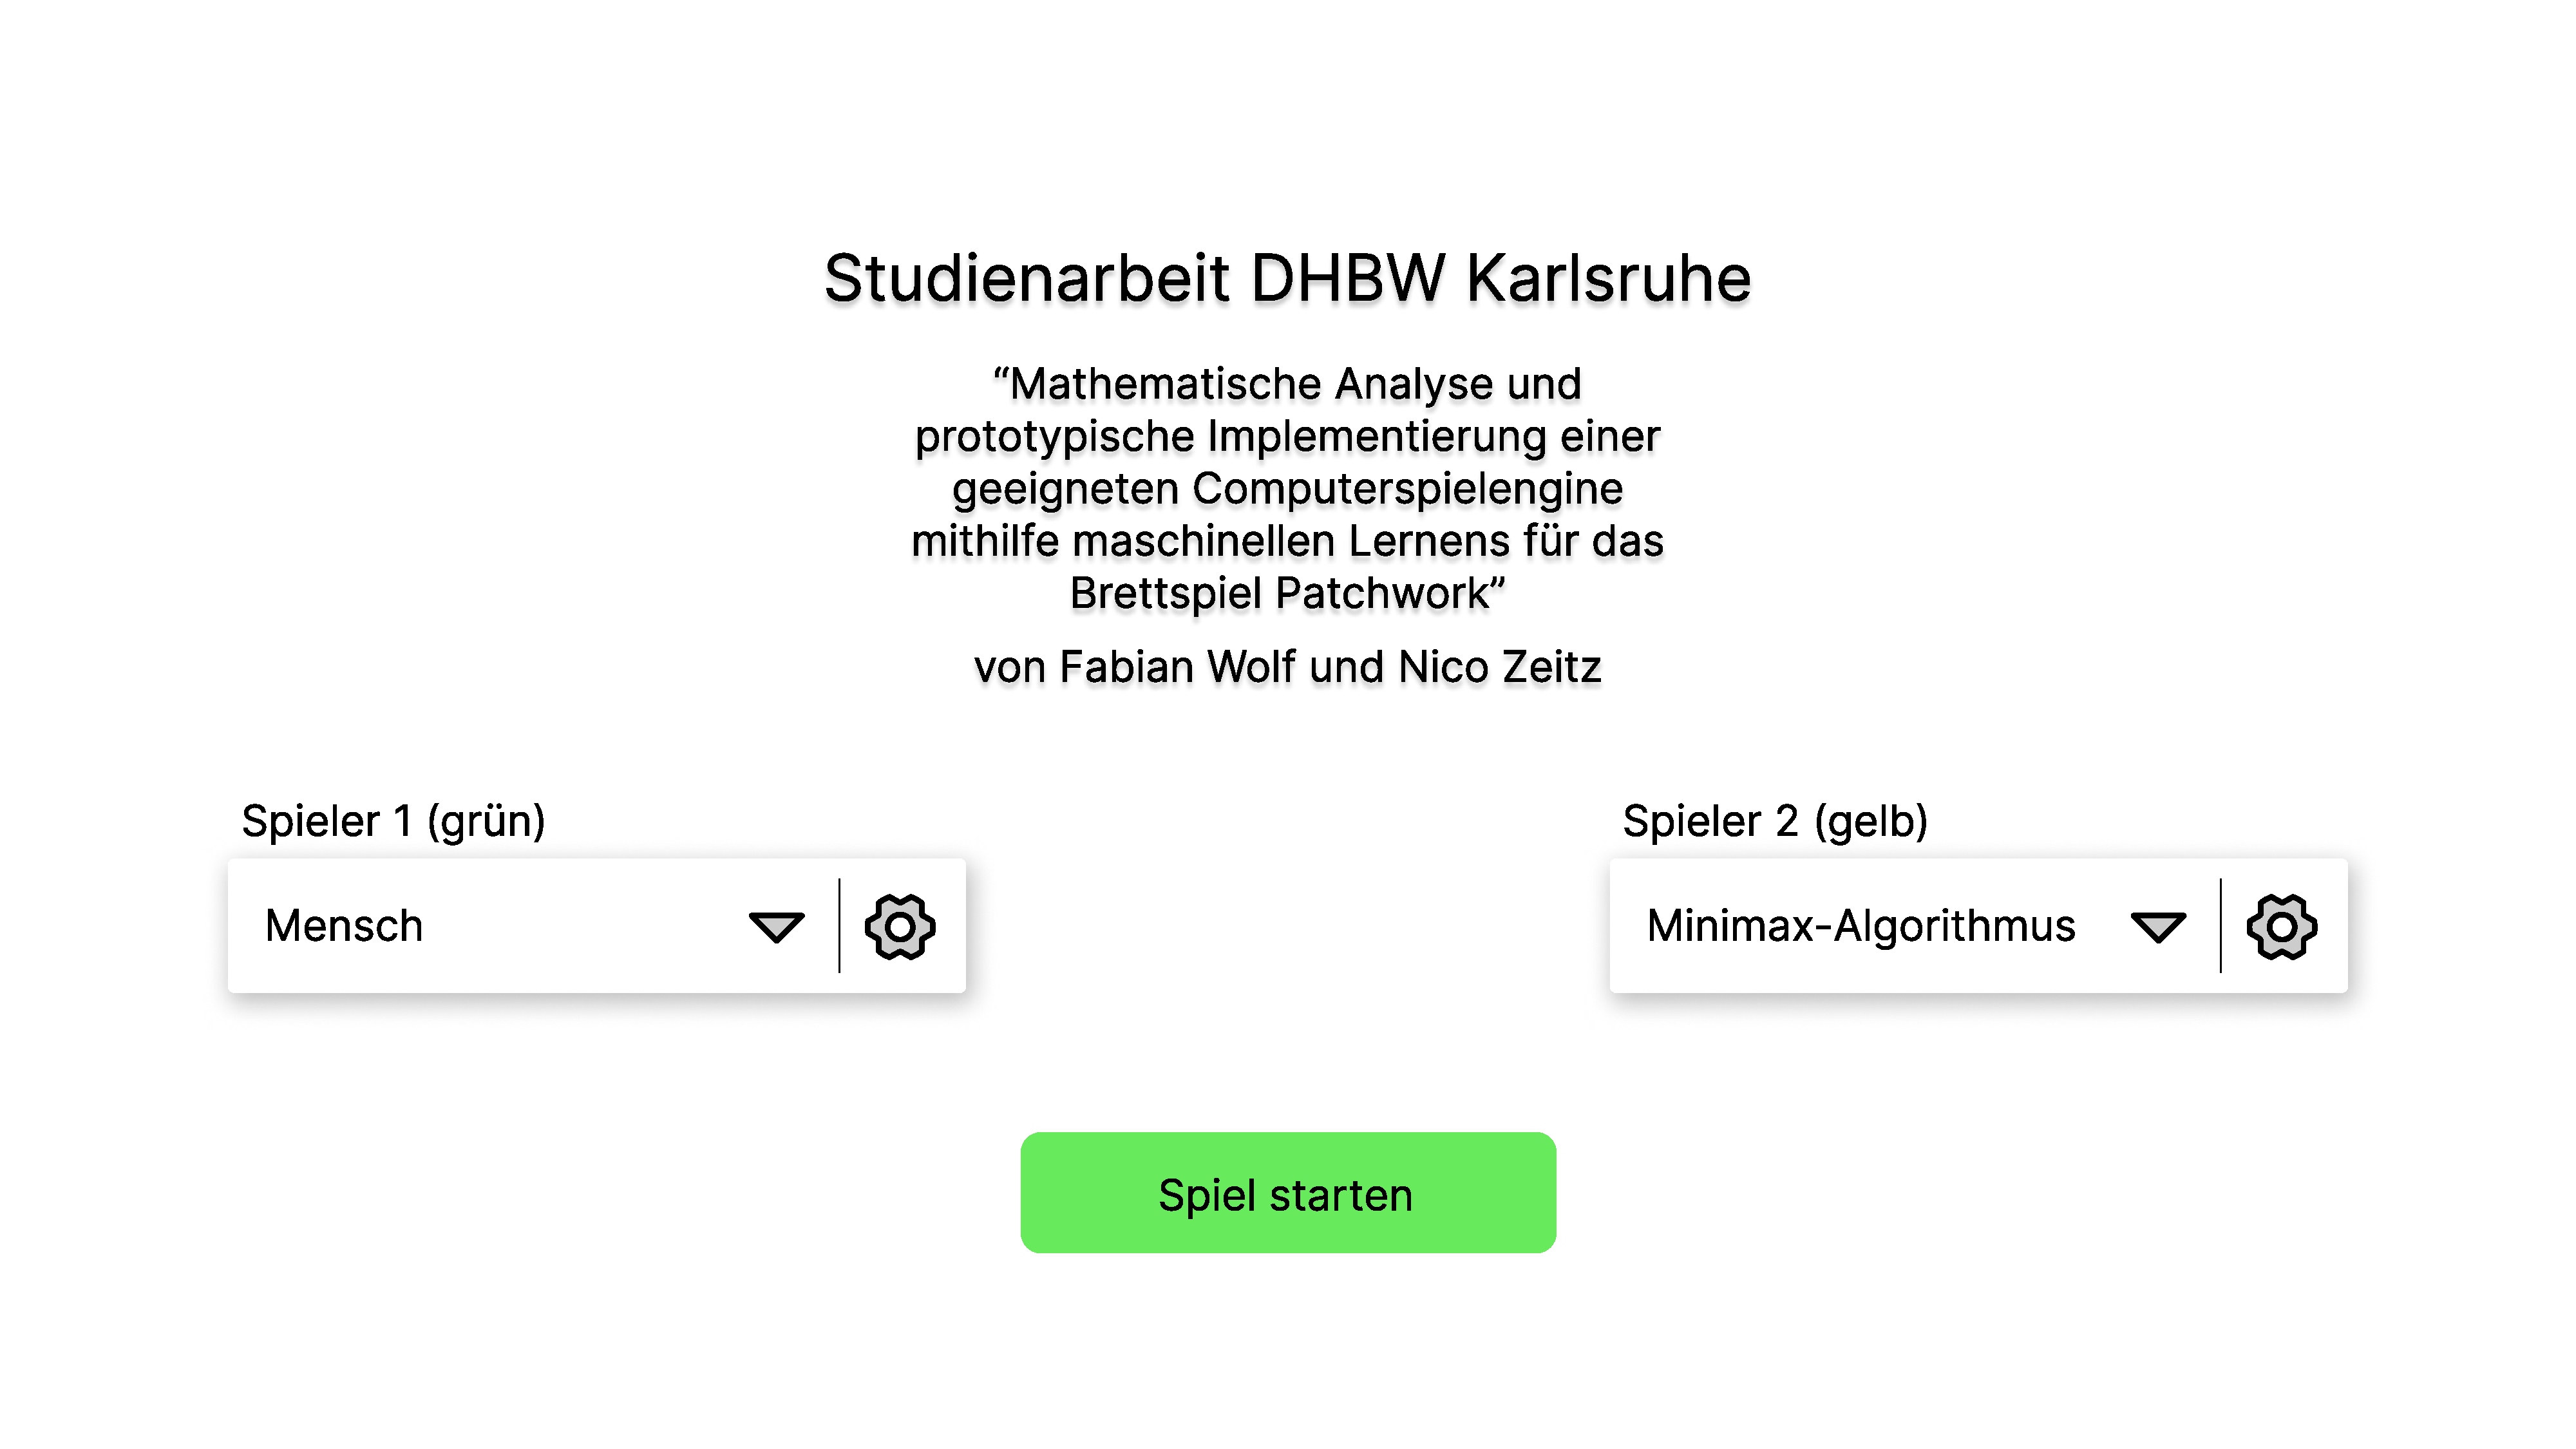
\includegraphics[width=\textwidth]{res/pictures/desig_main_ui.pdf}};
        \drawshadow{image}
    \end{tikzpicture}}
    \caption{Designentwurf vom Hauptmenü des Computerspiel}
    \label{fig:design-main-ui}
\end{figure}

In der Abbildung \ref{fig:design-main-ui} ist das Design des Hauptmenüs der interaktiven Benutzeroberfläche zu sehen. In dieser Oberfläche sollen alle möglichen Einstellungen für das Computerspiel getroffen werden können, wie die Auswahl der Computerspielengines und das Einstellen der Details der jeweiligen Computerspieler, um anschließend mit dem Knopf \enquote{Spiel starten} ein neues Patchwork-Spiel zu beginnen. Alle interaktiven Elemente, welche auf dieser Seite nur das Dropdown-Menü zur Auswahl der Spielertypen, das zugehörige Einstellungsmenü und der zuvor angesprochene Knopf sind, sollen auf den ersten Blick als Affordances vom Benutzer identifiziert werden können. Dazu werden bereits bestehende mentale Modelle der Benutzer genutzt, um eine bestimmte Bedienung der Software zu vermitteln. So wird die Assoziation, welche die Farbe Grün mit dem Start eines Prozesses verknüpft, verwendet und auf das Umfeld dieses Computerspiels umgemünzt und als Hintergrundfarbe für den Startknopf verwendet oder die weit verbreitete Analogie genutzt, dass hinter einem Zahnrad-Symbol ein Einstellungsmenü zu finden ist.

\begin{figure}[!ht]
    \centering
    \resizebox{\textwidth}{!}{\begin{tikzpicture}
        \node [inner sep=0pt,,outer sep=0pt,clip,rounded corners=0.15cm] (image) at (0,0) {
            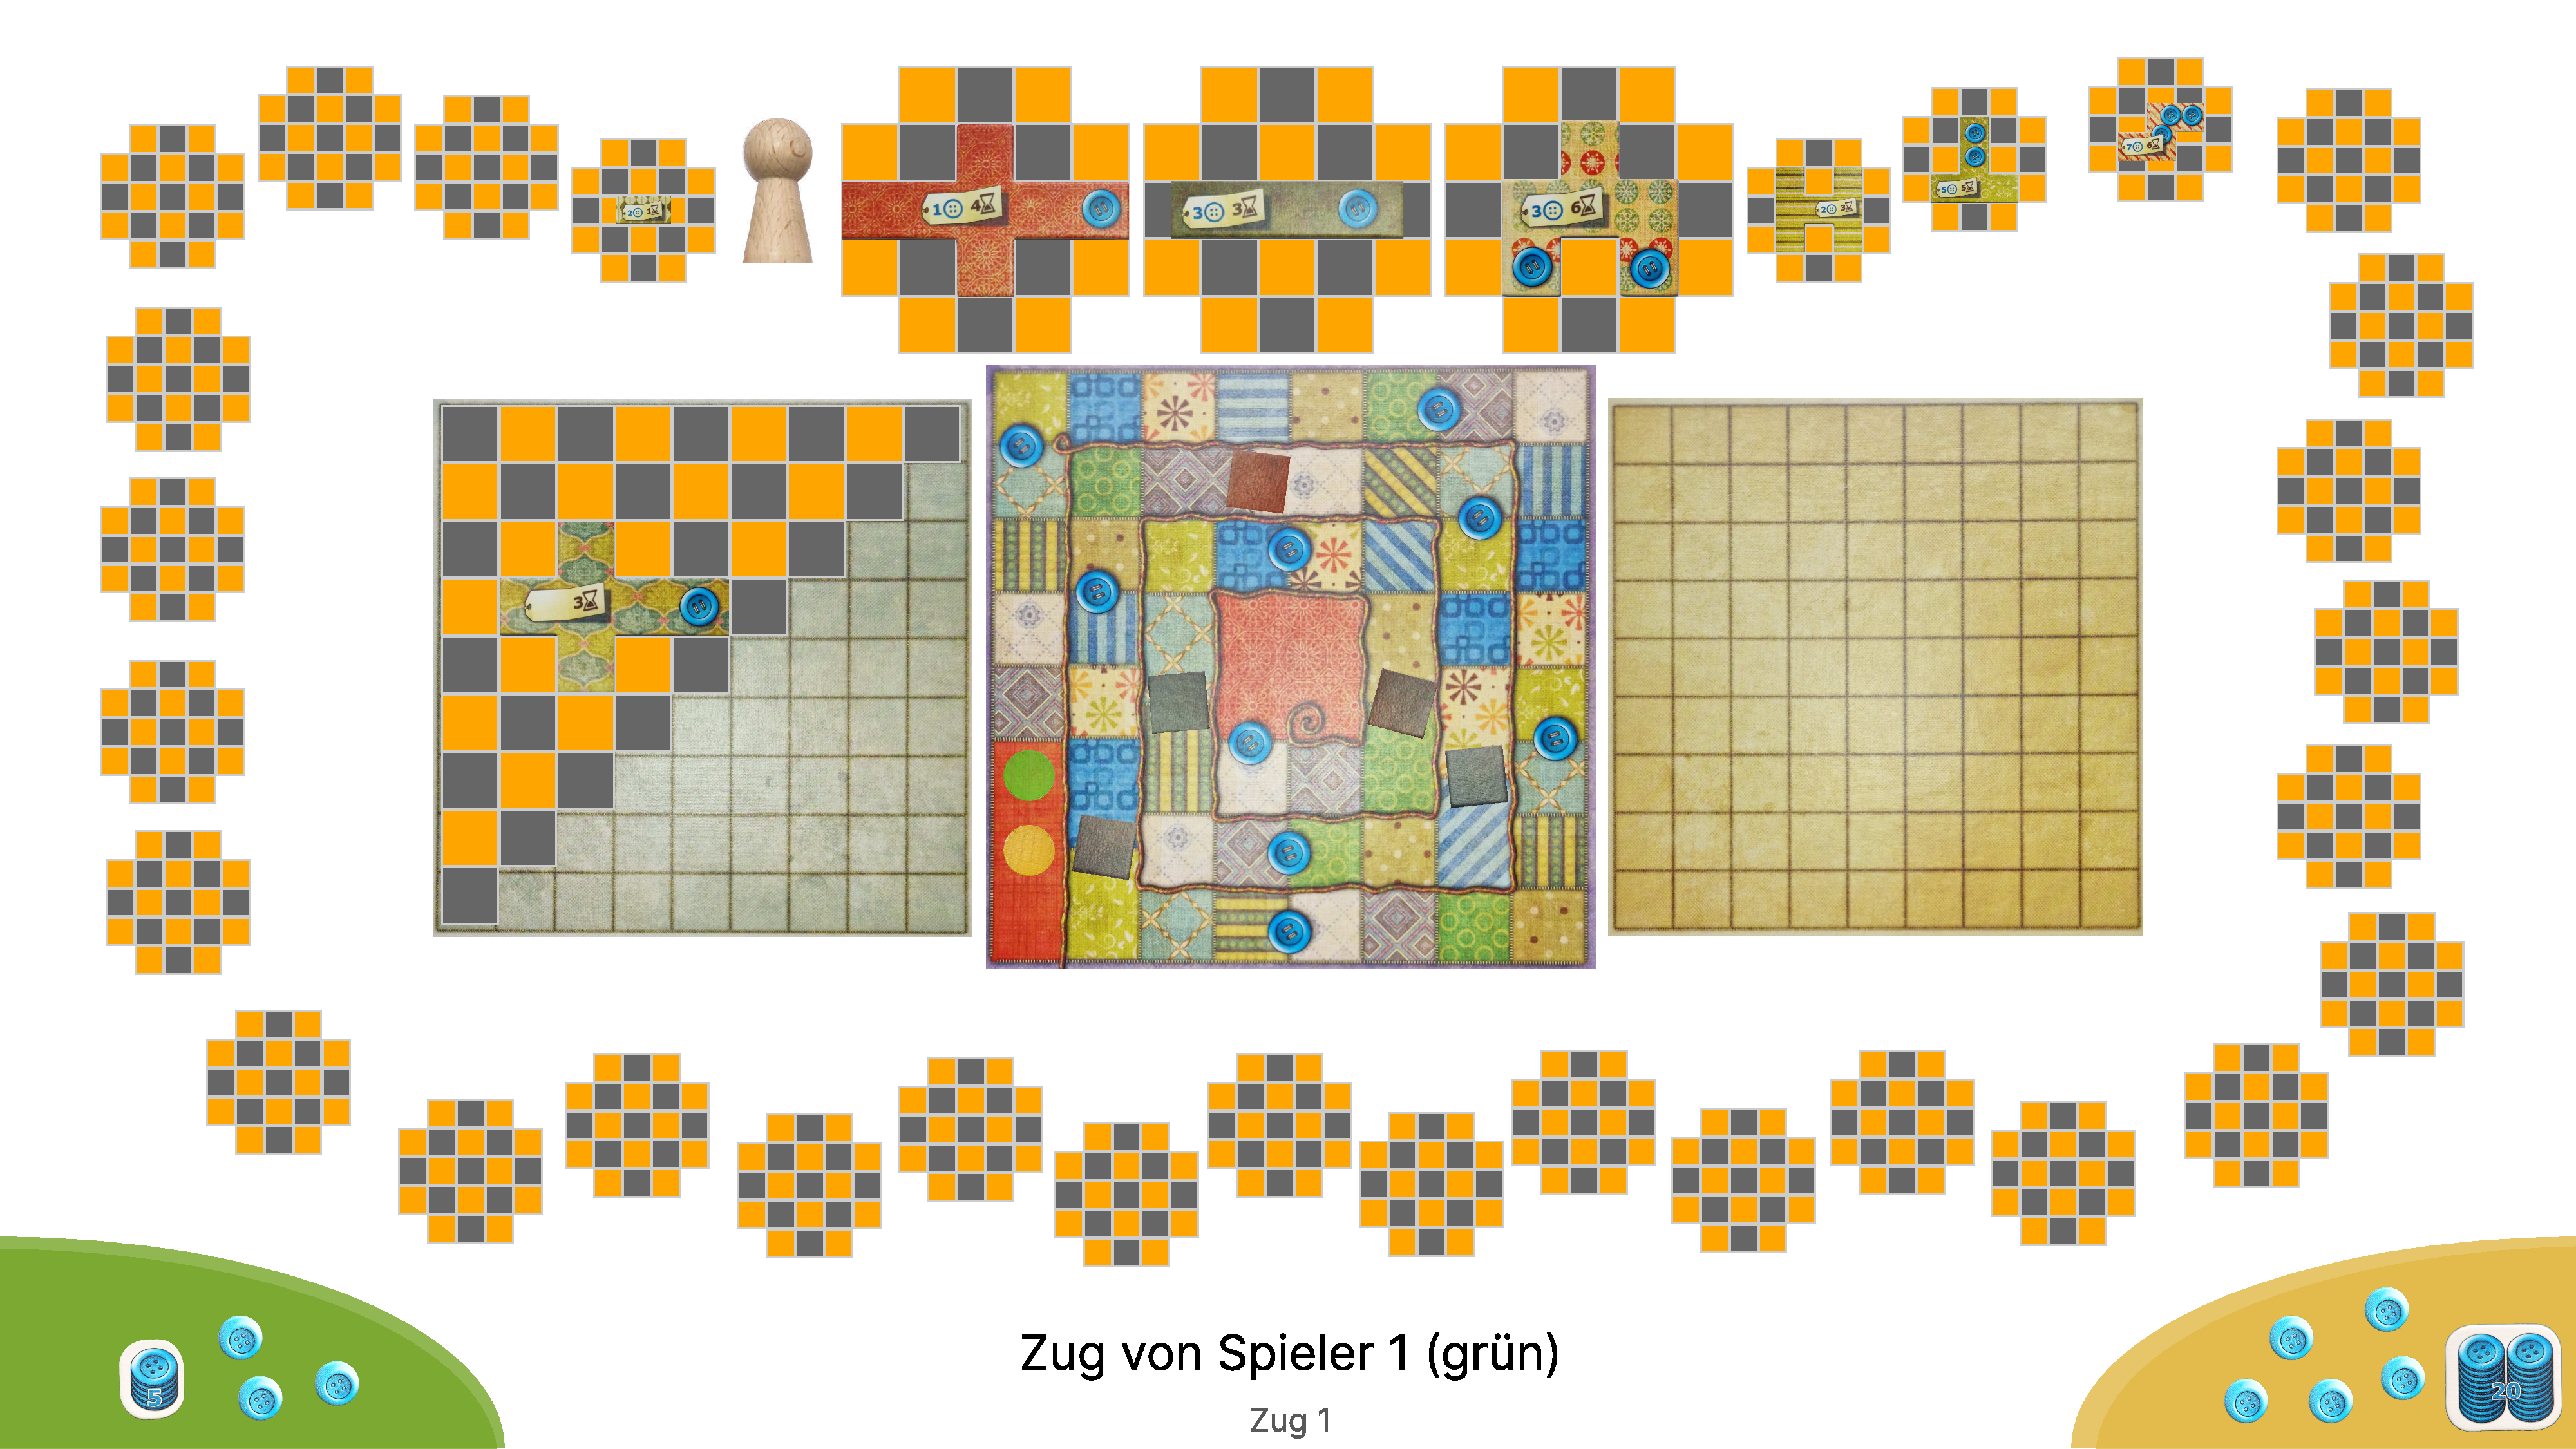
\includegraphics[width=\textwidth]{res/pictures/design_game_ui.pdf}};
        \drawshadow{image}
    \end{tikzpicture}}
    \caption{Designentwurf der grafische Benutzeroberfläche des Computerspiel}
    \label{fig:design-game-ui}
\end{figure}

Um das Brettspiel samt Spielgefühl bestmöglich auf das digitale Medium zu übertragen, wurde sich für das Design der Spieloberfläche, welche in der Abbildung \ref{fig:design-game-ui} zu sehen ist, am Spielaufbau des Brettspiels orientiert. Der Zeitplan liegt zentral in der Mitte der Oberfläche und wird an den Seiten von den Ablageplänen der beiden Spieler ergänzt.

Das Gesetz der Gleichheit bezüglich Farbe ausnutzend sind ist die Information, wie viel Knopfguthaben die Spieler haben, in den unteren Ecken der Oberfläche dargestellt. Um die Spielbretter herum sollen alle im Spiel befindlichen Flicken dargestellt werden, beziehungsweise in diesem Design die Platzhalter für diese Flicken. Hierbei sind die vom Spieler auswählbaren Flicken in voller Größe dargestellt, um sie hervorzuheben. Um diesen Aspekt zu erzielen, wird an dieser Stelle ebenfalls das Gesetz der Gleichheit, sowie das Gesetz der Nähe angewandt. Das letzte Gesetz wird hier außerdem dazu verwendet, um die Knöpfe zum Spiegeln und Rotieren der Flicken dem jeweiligen Flicken eindeutig zuzuordnen.

Insgesamt wurde bei der Darstellung aller Flicken die Gesetze der Nähe und der Ähnlichkeit verwendet: Alle Flicken zusammen wirken durch ihre räumliche Nähe als eine Einheit, während die Unterscheidung zwischen wählbar und nicht wählbar durch die Größe dargestellt wird. Durch die kleine Darstellung der nicht auswählbaren Flicken wird dieses Constraints dem Spieler grafisch vermittelt. Das Wirken als Einheit soll sich bei dem Platzieren eines Flickens, beziehungsweise dem Wechsel der auswählbaren Flicken, durch die Gesetze der Gleichzeitigkeit und der gemeinsamen Bewegung noch verstärkt werden. So soll die Flickeneinheit sich als Kreis drehen, bis die als nächstes auswählbaren Flicken an der richtigen Position in der oberen Mitte der Oberfläche angekommen sind. Dies muss durch eine langsame Transformation der Flicken passieren, damit diese Bewegung von deutlich mehr als fünf Objekten noch korrekt interpretiert werden kann. Die Interpretation dieser Bewegung sollte durch die ständige Wiederholung derselben, jedoch nach gewisser Zeit den Spielern sehr leichtfallen, was allerdings noch durch Spielerbefragungen verifiziert werden sollte.

Bei der Platzierung der Flicken soll auf das dem Benutzer durch zahlreiche andere Anwendungen bekannte Drag-and-Drop zur direkten Manipulation der Flicken zurückgegriffen werden. Dazu soll der transformierte Flicken mittels Mausklick ausgewählt werden können und wie im physischen Spiel auch zum eigenen Ablageplan bewegt werden und platziert werden können. Dasselbe Verfahren soll auch bei einer gewünschten Laufaktion des Spielers verwendet werden, was bedeutet, dass der Spieler einfach seine Spielfigur auf das korrekte Feld auf dem Zeitplan stellen muss, um die Aktion auszuführen, wodurch sich das Computerspiel wie die Vorlage spielt, eine Kenntnisübertragung möglich ist und ein ähnliches Spielgefühl entstehen kann.

\pagebreak

Unten in der Mitte sind die aktuellen Statusinformationen über das Spiel abgebildet, dort soll allerdings auch Spielbenachrichtigungen platzfinden, wie zum Beispiel der Aufforderung zur Platzierung des Spezialflickens, um die Einstiegshürde für neue Spieler weiter zu senken.

\begin{figure}[!ht]
    \centering
    \resizebox{\textwidth}{!}{\begin{tikzpicture}
        \node [inner sep=0pt,,outer sep=0pt,clip,rounded corners=0.15cm] (image) at (0,0) {
            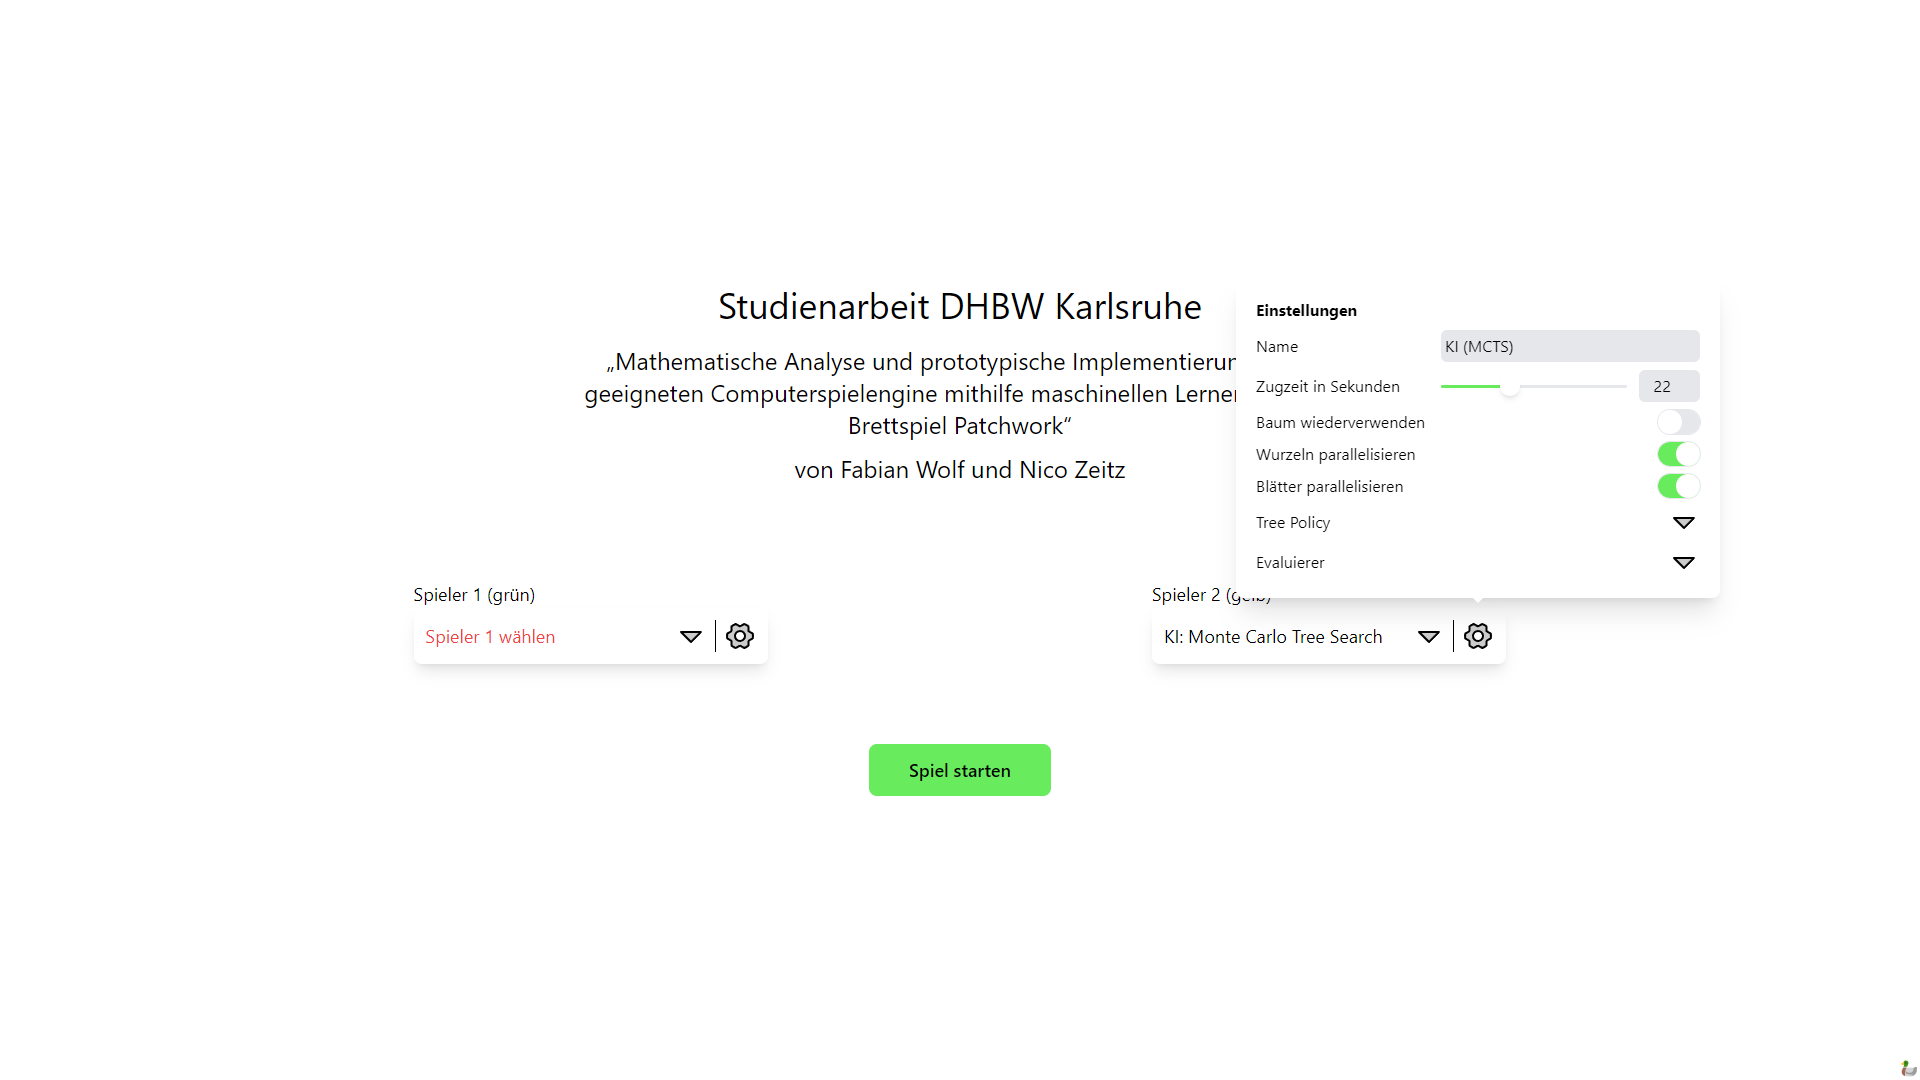
\includegraphics[width=\textwidth]{res/pictures/final_main_ui.png}};
        \drawshadow{image}
    \end{tikzpicture}}
    \caption{Umsetzung des Hauptmenüs des Computerspiel}
    \label{fig:final-main-ui}
\end{figure}

Bei Betrachtung der Umsetzung des Hauptmenüs in Abbildung \ref{fig:final-main-ui} im Vergleich zum Design in Abbildung \ref{fig:final-main-ui} lässt sich kein großer grafischer Unterschied feststellen. Das aufgeklappte Einstellungsmenü für die Computerspielengine \ac{MCTS}, verwendet bekannte Muster und Analogien zu Modifikation der Engine, wie zum Beispiel einem Slider zur annäherungsweisen Eingabe der Zugzeit der Engine, durch das Eingabefeld für genauere Eingabe erweitert. Diese Benutzeroberfläche des Hauptmenüs lässt sich laut ersten Testern intuitiv bedienen und wird als selbsterklärend beschrieben.

\pagebreak

\begin{figure}[!ht]
    \centering
    \resizebox{\textwidth}{!}{\begin{tikzpicture}
        \node [inner sep=0pt,,outer sep=0pt,clip,rounded corners=0.15cm] (image) at (0,0) {
            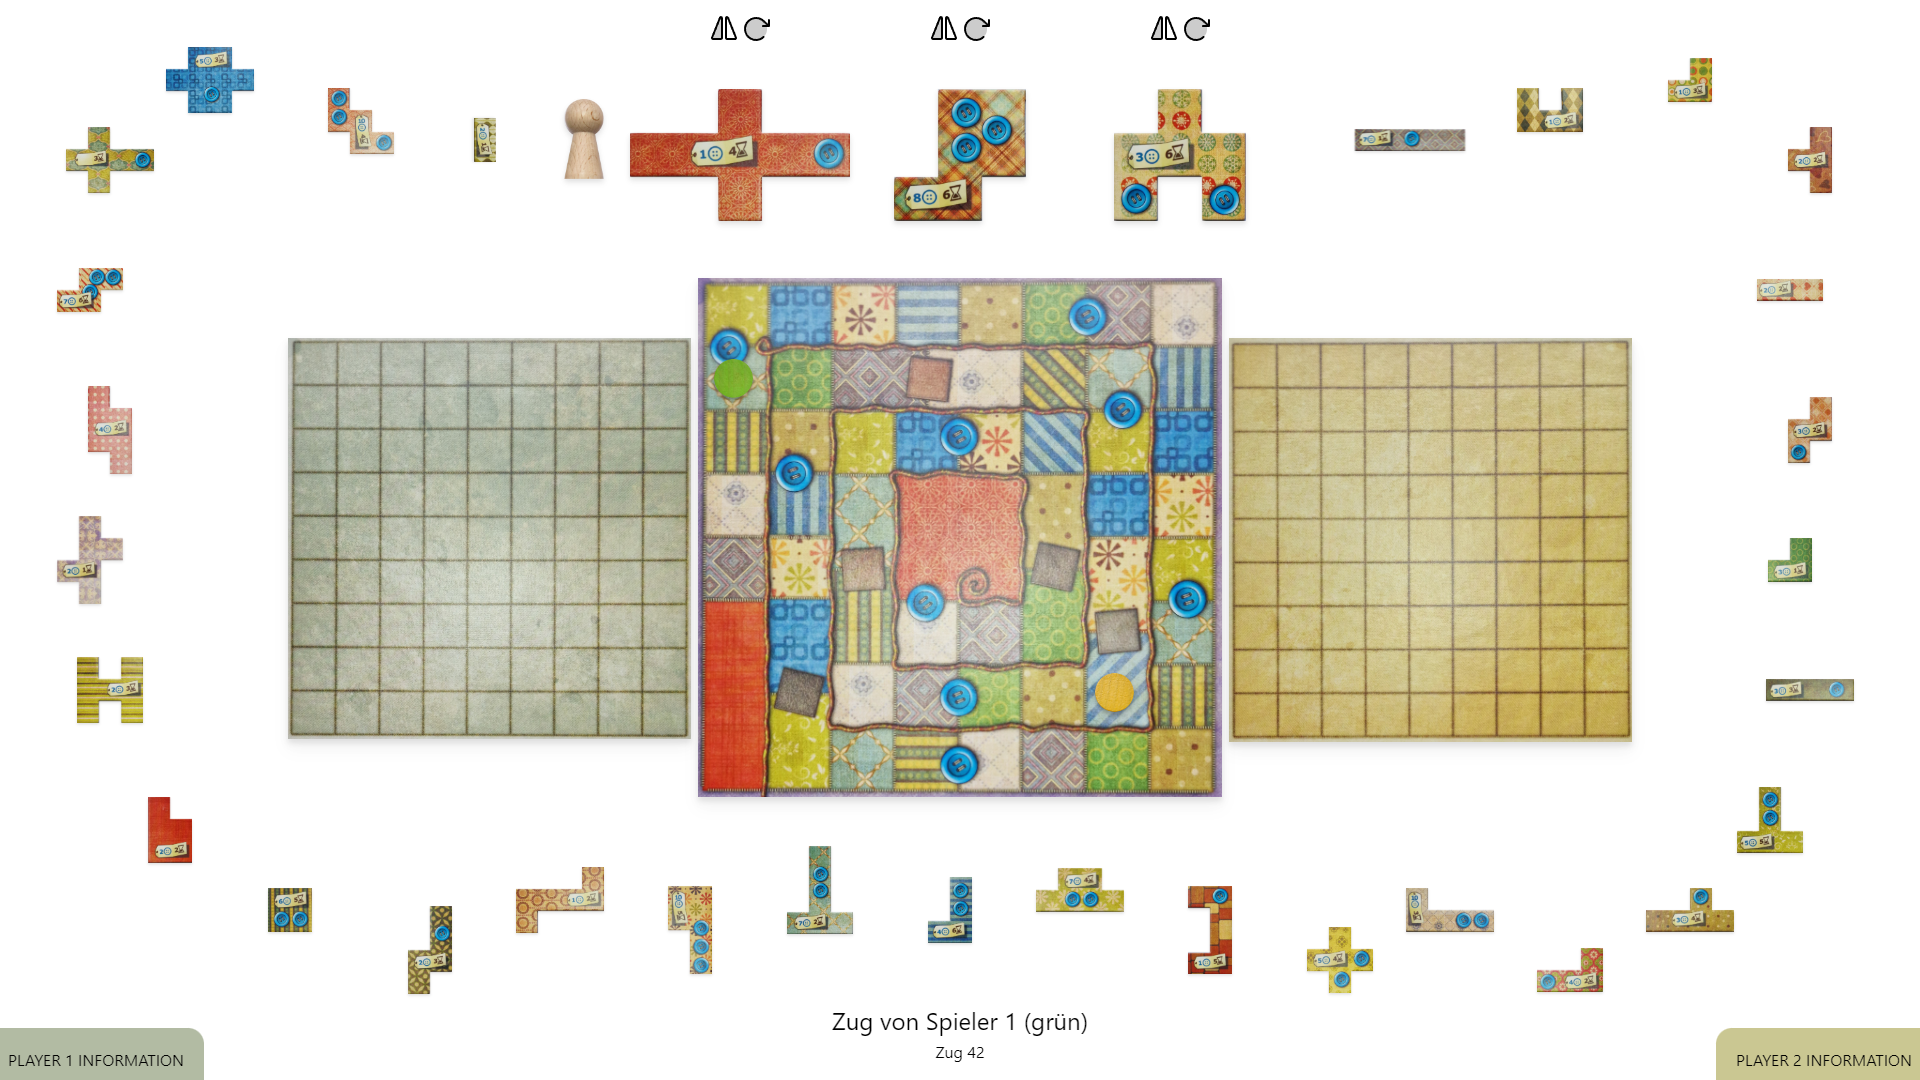
\includegraphics[width=\textwidth]{res/pictures/final_game_ui.png}};
        \drawshadow{image}
    \end{tikzpicture}}
    \caption{Umsetzung der grafische Benutzeroberfläche des Computerspiel}
    \label{fig:final-game-ui}
\end{figure}

Ebenso ist in der Umsetzung der Benutzeroberfläche des Computerspiels, in Abbildung \ref{fig:final-game-ui} zu sehen, deutlich das ursprüngliche Design zu erkennen. Die Flicken wirken in Kombination wie eine Kette, welche sich um die Spielbretter im Inneren zieht und werden durchaus als eine Einheit wahrgenommen. Ebenso erfolgreich wirkt die Unterscheidung zwischen auswählbaren Flicken, welche sich in der korrekten Größe für die Platzierung auf dem Ablageplan befinden, während die kleinen Flicken mit der Hälfte der Größe die gewünschte Unerreichbarkeit gegenüber den Spielern ausstrahlen. Die Zuordnung von Spielerinformationen zu den Ablageplänen funktioniert durch die gleiche Farbe ebenso erfolgreich. An dieser Stelle wird teilweise offensichtlich, dass die interaktive Benutzeroberfläche noch nicht fertiggestellt erscheint, da aufgrund von Zeitmangel die Implementierung nicht vollendet werden konnte.

Würde die interaktive Benutzeroberfläche wie zuvor beschreiben umgesetzt werden, sollte das Computerspiel deutlich einfacher und einsteigerfreundlicher sein, da viel Aspekte des Spiels automatisiert oder besser dargestellt werden können. Einige Beispiele hierfür sind das Verschieben der Flicken und Spielfigur, das einfache Erkennen welche Flicken zur Auswahl stehen und die Berechnung von Knopfeinkommen.